\setcounter{figure}{0}

\section{6th August 2023: Bad words}
\subsection*{Text: Proverbs 18:21}
  \begin{quote}
    [21] Death and life are in the power of the tongue, and those who love it
    will eat its fruits.
  \end{quote}
\subsection*{Notes}
\begin{itemize}
  \item{We use words to communicate with each other. Our words can build someone up or tear someone down. We know this from common sense, but also from Scripture.}
  \item{When God created us with the ability to talk and communicate, He set us apart from other creatures and also determined our purpose as humans. God created us with the ability to talk because talking is essential for forming relationships, and we are built for relationships. But because of sin, now our ability to talk have the potential to destroy relationships instead of to build up relationships.}
  \item{When we say negative things to people, the hurt we cause can cause lasting scars. The thing about words is that we can’t take them back after they leave our mouth. Our negative and hurtful words can cause irreparable damage to someone. }
  \item{Now, “the heart is deceitful above all things, and desperately sick” (Jer 17:9). And, “out of the abundance of the heart the mouth speaks” (Matthew 12:34). Ultimately, the reason why our words can hurt others is because our heart is sick. The words that come out of our mouth can only be as good as our heart, and the problem is that because of sin, our heart is sick. For example, angry words only come out from an angry heart.}
  \item{As James said, nobody can tame the tongue. But since the tongue is only a manifestation of the sin in our heart, when the heart is changed, then the tongue is can be subdued. And this change of heart is effected by God and His Holy Spirit.}
  \item{Most of the times, we hurt others with our words when others hurt us. We get angry when we perceive (correctly or incorrectly) other people sinning against us, then the angry words will come out. But this is where the gospel comes in. When we realise God’s forgiveness for us, then we can forgive others when they hurt us, and this would prevent us from saying hurtful words back to them. But all of this can only be done after God gives us a new heart.}
  % \item{\begin{figure}[H]
  %   \centering
  %   % 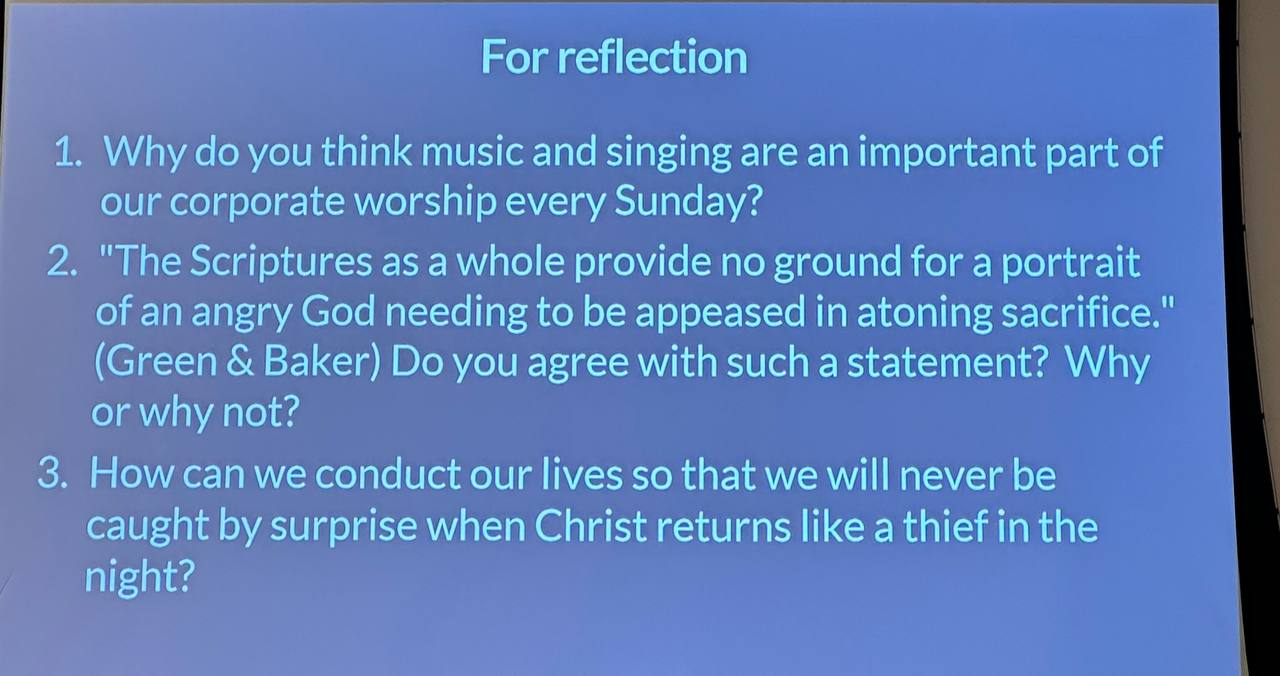
\includegraphics[width=0.8\textwidth, trim={0cm 0cm 0cm 0cm},clip]{Figures/marchSermon4Reflections.jpg}
  %   \includegraphics[width=0.8\textwidth, trim={0cm 0cm 0cm 0cm},clip]{example-image-a}
  %   \caption[]{Reflection questions for this sermon}
  %   \label{}
  % \end{figure}}
\end{itemize}